%Chapter 1
\chapter{Introduction and background}  %J.H Marais, C.J.R. Kriel
\pagenumbering{arabic} 
\setcounter{page}{1}
\section{Preamble}

\section{Background on deep level mining}

\subsection{Mining profitability}
Background on rising mining costs (energy, wages, etc), falling ore grades and Eskom tariffs.\cite{neingo2016trends}
%\begin{figure}
%	\centering
%	% GNUPLOT: LaTeX picture with Postscript
\begingroup
  \makeatletter
  \providecommand\color[2][]{%
    \GenericError{(gnuplot) \space\space\space\@spaces}{%
      Package color not loaded in conjunction with
      terminal option `colourtext'%
    }{See the gnuplot documentation for explanation.%
    }{Either use 'blacktext' in gnuplot or load the package
      color.sty in LaTeX.}%
    \renewcommand\color[2][]{}%
  }%
  \providecommand\includegraphics[2][]{%
    \GenericError{(gnuplot) \space\space\space\@spaces}{%
      Package graphicx or graphics not loaded%
    }{See the gnuplot documentation for explanation.%
    }{The gnuplot epslatex terminal needs graphicx.sty or graphics.sty.}%
    \renewcommand\includegraphics[2][]{}%
  }%
  \providecommand\rotatebox[2]{#2}%
  \@ifundefined{ifGPcolor}{%
    \newif\ifGPcolor
    \GPcolortrue
  }{}%
  \@ifundefined{ifGPblacktext}{%
    \newif\ifGPblacktext
    \GPblacktextfalse
  }{}%
  % define a \g@addto@macro without @ in the name:
  \let\gplgaddtomacro\g@addto@macro
  % define empty templates for all commands taking text:
  \gdef\gplbacktext{}%
  \gdef\gplfronttext{}%
  \makeatother
  \ifGPblacktext
    % no textcolor at all
    \def\colorrgb#1{}%
    \def\colorgray#1{}%
  \else
    % gray or color?
    \ifGPcolor
      \def\colorrgb#1{\color[rgb]{#1}}%
      \def\colorgray#1{\color[gray]{#1}}%
      \expandafter\def\csname LTw\endcsname{\color{white}}%
      \expandafter\def\csname LTb\endcsname{\color{black}}%
      \expandafter\def\csname LTa\endcsname{\color{black}}%
      \expandafter\def\csname LT0\endcsname{\color[rgb]{1,0,0}}%
      \expandafter\def\csname LT1\endcsname{\color[rgb]{0,1,0}}%
      \expandafter\def\csname LT2\endcsname{\color[rgb]{0,0,1}}%
      \expandafter\def\csname LT3\endcsname{\color[rgb]{1,0,1}}%
      \expandafter\def\csname LT4\endcsname{\color[rgb]{0,1,1}}%
      \expandafter\def\csname LT5\endcsname{\color[rgb]{1,1,0}}%
      \expandafter\def\csname LT6\endcsname{\color[rgb]{0,0,0}}%
      \expandafter\def\csname LT7\endcsname{\color[rgb]{1,0.3,0}}%
      \expandafter\def\csname LT8\endcsname{\color[rgb]{0.5,0.5,0.5}}%
    \else
      % gray
      \def\colorrgb#1{\color{black}}%
      \def\colorgray#1{\color[gray]{#1}}%
      \expandafter\def\csname LTw\endcsname{\color{white}}%
      \expandafter\def\csname LTb\endcsname{\color{black}}%
      \expandafter\def\csname LTa\endcsname{\color{black}}%
      \expandafter\def\csname LT0\endcsname{\color{black}}%
      \expandafter\def\csname LT1\endcsname{\color{black}}%
      \expandafter\def\csname LT2\endcsname{\color{black}}%
      \expandafter\def\csname LT3\endcsname{\color{black}}%
      \expandafter\def\csname LT4\endcsname{\color{black}}%
      \expandafter\def\csname LT5\endcsname{\color{black}}%
      \expandafter\def\csname LT6\endcsname{\color{black}}%
      \expandafter\def\csname LT7\endcsname{\color{black}}%
      \expandafter\def\csname LT8\endcsname{\color{black}}%
    \fi
  \fi
    \setlength{\unitlength}{0.0500bp}%
    \ifx\gptboxheight\undefined%
      \newlength{\gptboxheight}%
      \newlength{\gptboxwidth}%
      \newsavebox{\gptboxtext}%
    \fi%
    \setlength{\fboxrule}{0.5pt}%
    \setlength{\fboxsep}{1pt}%
\begin{picture}(7200.00,5040.00)%
    \gplgaddtomacro\gplbacktext{%
      \colorrgb{0.50,0.50,0.50}%
      \put(1078,924){\makebox(0,0)[r]{\strut{}$8500$}}%
      \colorrgb{0.50,0.50,0.50}%
      \put(1078,1269){\makebox(0,0)[r]{\strut{}$9000$}}%
      \colorrgb{0.50,0.50,0.50}%
      \put(1078,1615){\makebox(0,0)[r]{\strut{}$9500$}}%
      \colorrgb{0.50,0.50,0.50}%
      \put(1078,1960){\makebox(0,0)[r]{\strut{}$10000$}}%
      \colorrgb{0.50,0.50,0.50}%
      \put(1078,2306){\makebox(0,0)[r]{\strut{}$10500$}}%
      \colorrgb{0.50,0.50,0.50}%
      \put(1078,2651){\makebox(0,0)[r]{\strut{}$11000$}}%
      \colorrgb{0.50,0.50,0.50}%
      \put(1078,2997){\makebox(0,0)[r]{\strut{}$11500$}}%
      \colorrgb{0.50,0.50,0.50}%
      \put(1078,3342){\makebox(0,0)[r]{\strut{}$12000$}}%
      \colorrgb{0.50,0.50,0.50}%
      \put(1078,3688){\makebox(0,0)[r]{\strut{}$12500$}}%
      \colorrgb{0.50,0.50,0.50}%
      \put(1078,4033){\makebox(0,0)[r]{\strut{}$13000$}}%
      \colorrgb{0.50,0.50,0.50}%
      \put(1078,4379){\makebox(0,0)[r]{\strut{}$13500$}}%
      \colorrgb{0.50,0.50,0.50}%
      \put(1210,704){\makebox(0,0){\strut{}$2011$}}%
      \colorrgb{0.50,0.50,0.50}%
      \put(2329,704){\makebox(0,0){\strut{}$2012$}}%
      \colorrgb{0.50,0.50,0.50}%
      \put(3447,704){\makebox(0,0){\strut{}$2013$}}%
      \colorrgb{0.50,0.50,0.50}%
      \put(4566,704){\makebox(0,0){\strut{}$2014$}}%
      \colorrgb{0.50,0.50,0.50}%
      \put(5684,704){\makebox(0,0){\strut{}$2015$}}%
      \colorrgb{0.50,0.50,0.50}%
      \put(6803,704){\makebox(0,0){\strut{}$2016$}}%
    }%
    \gplgaddtomacro\gplfronttext{%
      \csname LTb\endcsname%
      \put(176,2651){\rotatebox{-270}{\makebox(0,0){\strut{}y axis label}}}%
      \put(4006,374){\makebox(0,0){\strut{}x axis label}}%
      \put(4006,4709){\makebox(0,0){\strut{}Title}}%
      \csname LTb\endcsname%
      \put(4701,173){\makebox(0,0)[r]{\strut{}'HarmonyCost.dat'}}%
    }%
    \gplbacktext
    \put(0,0){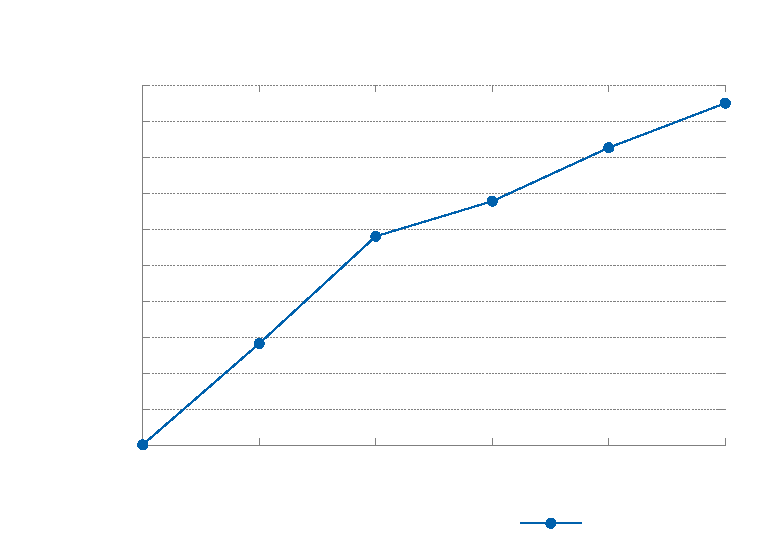
\includegraphics{Graphs/introduction}}%
    \gplfronttext
  \end{picture}%
\endgroup

%\end{figure} 


\subsection{Mining systems and energy}
Focus an mine electrical energy users. Compressed air and its inefficiencies
\subsection{Need to improve service delivery}
\section{Mining compressed air systems}v
	\subsection{Compressed air in operation}
	\subsection{Characteristic inefficiencies}
	\subsection{Inefficiency identification methods}
	\subsection{Instrumentation and measurements}
\section{Simulations in industry}

Continuous improvements in computing hardware has led to major advancement in software technology. Consequently the use of computational simulation has become an increasingly valuable tool for many industries.\cite{kocsis2003integration} \par 

Simulation has many benefits besides prediction. Some of advantages discussed in Banks' \textit{ Handbook of simulation: principles, methodology, advances, applications, and practice} are: \cite{banks1998handbook}:
\begin{itemize}
	\item The ability to test new policies, operating procedures and methods without causing a disruption to the actual system.
	\item Identify problems in complex systems by gathering insight in the interactions within the system.
	\item Simulation allows you to compress or expand time to investigate phenomena thoroughly
	\item With simulation the limits and constraints within a system can be determined.
	\item Stimulation can help build consensus with regard to proposed designs or modifications.
\end{itemize}

\subsection{Computer software}
\paragraph{KY Pipe}
Ky pipe background. \cite{Wood1993KYPipe}
\paragraph{Simulation toolbox}
STB background.
\section{Problem statement and objectives}
\section{Dissertation overview}